\documentclass[11pt]{article}
\usepackage{cs170}
\usepackage{tikz}
\usetikzlibrary{positioning}


\def\title{Homework 9}
\def\duedate{3/22/2024, at 10:00 pm (grace period until 4/1/2024 11:59pm)} 


\begin{document}
\maketitle

Due \textbf{\duedate}

\question{Study Group}
List the names and SIDs of the members in your study group.
If you have no collaborators, you must explicitly write ``none''.

\begin{solution} I worked on this homework with the following collaborators:
\begin{itemize}
    \item Lakshya Nagal, SID: 3037935253 
\end{itemize}
\end{solution}

\question{Applications of Max-Flow Min-Cut}
Review the statement of max-flow min-cut theorem and prove the following two statements. 
\begin{subparts}
 \subpart   
Let $G = (L \cup R,E)$ be a unweighted bipartite graph\footnote{A bipartite graph $G = (L \cup R, E)$ is defined as a graph that can be partitioned into two disjoint sets of vertices (i.e. $L$ and $R$) such that no two vertices within the same set are adjacent.  
}. Then $G$ has a $L$-perfect
matching (a matching\footnote{A matching is defined as a set of edges that share no common vertices.} with size $|L|$) if and only if, for every set $X \subseteq L$, $X$ is connected to at least $|X|$ vertices
in $R$. You must prove both directions. 

\textit{Hint: Use the max-flow min-cut theorem on the cut that forms $X$ and $L \ \backslash \ X$.}\\
\begin{solution}
    If $G$ has a $L$-perfect matching, then by the definition of perfect matching, there are vertices 
    in $X \subseteq L$ such that they are connected to at least $|X|$ distinct vertices in $R$.
    For the opposite direction, consider adding node $s$ and $t$ to $L$ and $R$ respectively and let all the edges have capacity of 1.
    \begin{center}
        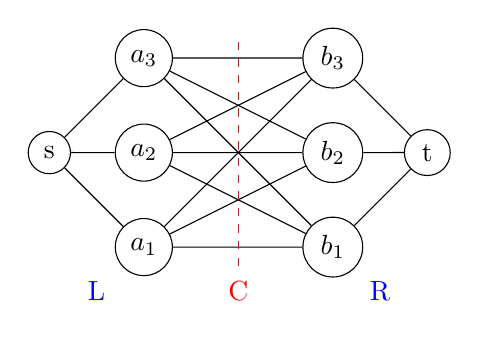
\begin{tikzpicture}[scale=1.2]
            % Define vertices
            \foreach \i in {1,...,3}{
                \node[circle, draw] (a\i) at (0,\i) {$a_\i$};
                \node[circle, draw] (b\i) at (2,\i) {$b_\i$};
            }
            % Add nodes S and T
            \node[circle, draw] (S) at (-1,2) {s};
            \node[circle, draw] (T) at (3,2) {t};
            % Draw edges
            \foreach \i in {1,...,3}{
                \foreach \j in {1,...,3}{
                \draw (a\i) -- (b\j);
                }
            }
            % Connect nodes S and T to vertices on their respective sides
            \foreach \i in {1,...,3}{
                \draw (S) -- (a\i);
                \draw (T) -- (b\i);
            }
            \draw[red, dashed] (1,0.8) -- (1,3.2);
            \node[red, below=2pt] at (1,0.8) {C};
            \node[blue, below=2pt] at (-0.5,0.8) {L};
            \node[blue, below=2pt] at (2.5,0.8) {R};
          \end{tikzpicture}
    \end{center}
    Let $\color{red} C$ be the the minimum cut. If $\color{red} C$ is the minimum
    cut, then according to the max-flow min-cut theorem, this means that the
    maximum flow in the graph is also at least the size of $L$. Since the maximum flow in the graph is at least the size of $L$, this implies that there is enough capacity to match each vertex in $L$ to a unique vertex in $R$. 
    Therefore, an $L$-perfect matching must exist in the graph.
\end{solution}
\newpage
\subpart
Let $G$ be an unweighted directed graph and $s,t \in V$ be two distinct vertices. Then the maximum number of
edge-disjoint $s$-$t$ paths equals the minimum number of edges whose removal disconnects $t$ from
$s$ (\textit{i.e.}, no directed path from $s$ to $t$ after the removal). 
\begin{solution}
    To approach this problem, we assign a capacity of 1 to each edge and connect the vertices of graphs L and R to nodes s and t, respectively. This allows us to reframe the problem as an integer max flow problem.
    In an unweighted graph, the max flow corresponds to the maximum number of edge-disjoint paths. Moreover, the minimum number of edges required to disconnect t and s is equivalent to the capacity of our min cut. Therefore, the max flow value must be identical to the min cut value.
\end{solution}
\end{subparts}

\newpage
\question{The Matching Game}
The matching game is played over the complete weighted bipartite graph $G(V, E)$ with positive edge weights $w_e$. The edge player plays an edge $e \in E$ while the vertex player plays a vertex $v \in V$ and if $v$ is one of the endpoints of $e$ (we will denote this by $v \in e$), the edge player pays $w_e$ to the vertex player. The edge player would like to minimize the amount they have to pay the vertex player, while the vertex player wants to maximize their earnings.
\begin{subparts}
\subpart If the vertex player plays a uniformly random vertex what is the best response for the edge player?\\
\begin{solution}
    The best response from the edge player would be to choose a pure strategy and choose the lightest weighted edge.
\end{solution}
\subpart If the edge player plays a uniformly random edge from the minimum weight matching, what is the best response for the vertex player?\\
\begin{solution}
    In this scenario, the vertex player wants to earn as much as possible. So, the best thing for them to do is to employ a pure strategy that chooses a vertex that's connected to the heaviest edge in the minimum weight matching. Since all edges in the minimum weight matching have an equal chance of being chosen, we always go for the heaviest edge's endpoint to maximize our earnings.
\end{solution}
\subpart Are these two strategies optimal for this game? If so, provide a brief justification. If not, write the 2 LP's corresponding to the edge player and vertex player, respectively, such that solving them yields each player's optimal strategy. You do not need to write these LP's in canonical form; however, it should be clear what all the constraints are.
\begin{solution}
    (b) is not an optimal strategy since as this gives a chance for the vertex player to reap high earnings. A more optimal strategy is the following:\\
    For edge player:
    \begin{align*}
        min_c ~ max_r &\sum_{e\in E} c_ew_e(r_{V_l} + r_{V_R})\\
        \text{s.t } &\sum c_i = 1\\
        &\sum r_j = 1\\
        & c_i, r_j \geq 0
    \end{align*}
    For vertex player:
    \begin{align*}
        max_r ~ min_c &\sum_{e\in E} c_ew_e(r_{V_l} + r_{V_R})\\
        \text{s.t } &\sum c_i = 1\\
        &\sum r_j = 1\\
        & c_i, r_j \geq 0
    \end{align*}
\end{solution}
\end{subparts}

\end{document}